%!TEX root = ../thesis.tex
\chapter{Design \& Implementation}

	Development of a graphical user interface for libmapper creates a unique challenge. Obviously such an interface is a practical tool, and should function as such, yet it also must work in concert with DMIs which are inherently designed for abstract and creative use. For the purposes of this project, the assumed solution to this innate paradox is to provide the user with multiple independent modes of control.  This assumption was made based on experiences with prior user interfaces for libmapper (vizmapper, max mapperGUI): for each interface users reported excellent functionality for certain use cases, and poor functionality for others. Libmapper itself is an extremely flexible API that makes few assumptions as to the network of devices and signals, nor how they are being mapped. It is fitting that a GUI for libmapper would be equally as flexible. In lieu of a single perfect solution for network visualization an interactivity, providing users with various independent solutions provided a good compromise.
	
\section{Design Background}

\begin{figure}[ht]
\centering
	\scalebox{0.42}{\hbox{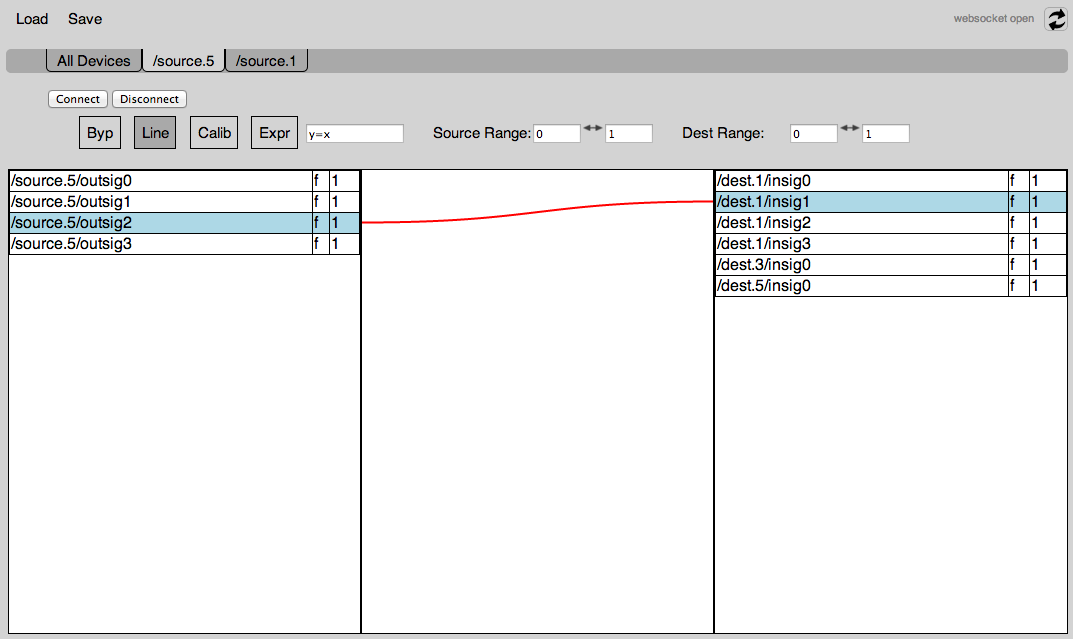
\includegraphics{figures/webmapper}}}
\caption{The webmapper interface}
\label{fig:webmapper}
\end{figure}

Work on this project began with a moderately featured, little used GUI for libmapper known as ``webmapper.'' Webmapper was created at IDMIL as an attempt to replace the Max/MSP GUI, as the result of limitations described in section \ref{sec:similar_interfaces}, the principle among which being the cross-platform incompatibility of Max/MSP. It was thought that an interface built for a web browser would greatly simplify the process of creating an cross-compatibility with all major operating systems and even mobile devices. 

Webmapper utilizes the Python bindings for libmapper by registering an admistrative monitor that can communicate with and control whichever libmapper network on which it happens to be. The monitor can create and modify connections or link, as well as query the network as to what devices, signals, links and connections are present. The webmapper code creates a simple HTTP server and attempts to open Google Chrome\footnote{Chrome Browser. [Online]. Available: \url{https://www.google.com/intl/en/chrome/browser/}. Accessed July 17, 2013} on the host computer. If Google Chrome is not present, the user must navigate directly to the server using the web address \url{localhost:50000}. The monitor communicates with the libmapper network and the local server, the browser is able to see messages the monitor ``posts'' to the server (such as `new device') and respond to them appropriatley. The browser in turn can send messages to the server (like `connect') that will propogate up to libmapper itself, eventually resulting in a message cascading back down to the browser reflecting the change to the network (such as `new connection'). 

The interface itself is written for a web browser using the scriting language JavaScript\footnote{JavaScript | MDN. [Online]. Available: \url{https://developer.mozilla.org/en-US/docs/Web/JavaScript}. Accessed July 17, 2013} to control web-standard HyperText Markup Language (HTML) elements and Cascading Style Sheets (CSS). The JavaScript code stores four main data structures: devices, links, connections and signals. The code never directly modifies any of this data, and instead it waits for messages relayed from libmapper. For example, if a user creates a new link, webmapper does not add a link to the links array but simply sends a message to the network. If it receives a `new link' message back, only then does it add the new link to the array. This is done to ensure that the data structures within webmapper always reflect what is actually present on the network in the case that messages are dropped, an error occurs, etc.

Figure \ref{fig:webmapper} shows the look of the interface before the work of this project began. Users are able to perform all libmapper functions: connecting, linking and modifying connections, but only the simplest of feature sets is included. For example, in order to form a connection the user must click on a source signal, click on a destination signal and then click on a button labelled ``connect.'' Many useful features of the Max/MSP interface, such as column headers, table sorting, drawing connections and search filtering are not present.

\section{Development of a Flexible Interface}
	
Prior GUIs for libmapper have been successfully used for some time, but all fail for one reason: they cannot accomidate all possible use-cases of libmapper. 
	%Needs to be adaptable, show any metadata

\subsection{List view}
\label{sec:list_view}

The first implemented, and thus far most functional view mode for the GUI is the ``list'' view. Based heavily on the Max/MSP GUI described in section \ref{sec:similar_interfaces}, 

\subsection{Grid view}
\subsection{Hive plot}
\subsection{Cluster view (vizmapper)}

\section{Control Features}
\subsection{Creating Connections/Links}
\subsection{Modifying Signals}

\section{The Model-View-Controller}

	Because a modular design is desired, the Model-View-Controller (MVC) metaphor for structuring software applications as described in [KrasnerPope88] was used as a general framework for structuring the application. In fact, the whole scale swapping in and out of independent visual modes can be thought of as a quintessential implementation of MVC. 
	
\subsection{The Model}

	The model consists of an abstract copy of the network, residing on the local machine. Independent views can consult this data, but cannot directly modify it.

\subsection{Controller-View Pairs}

\section{Graphical Design}
	wiggly arrows
\subsection{Typography}

\begin{figure}[ht]
\centering
	\scalebox{0.4}{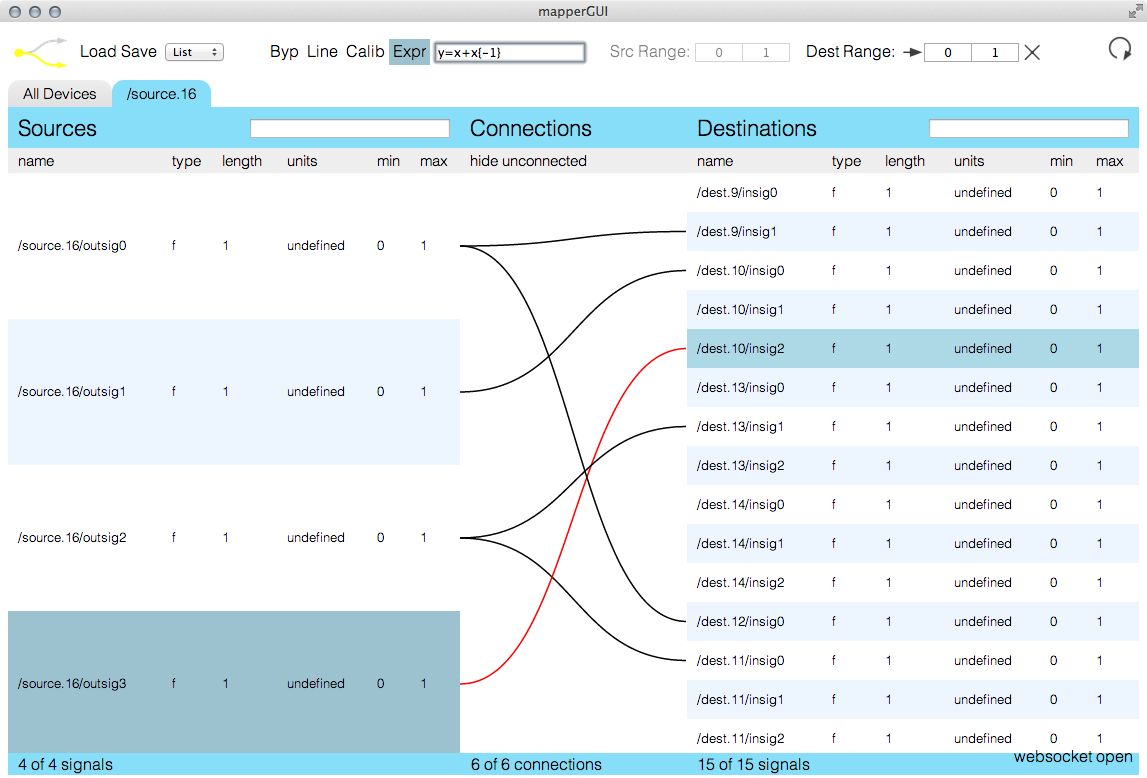
\includegraphics{figures/final_list}}
\caption{The list view after redesign}
\label{fig:final_list}
\end{figure}

\begin{figure}[ht]
\centering
	\scalebox{0.4}{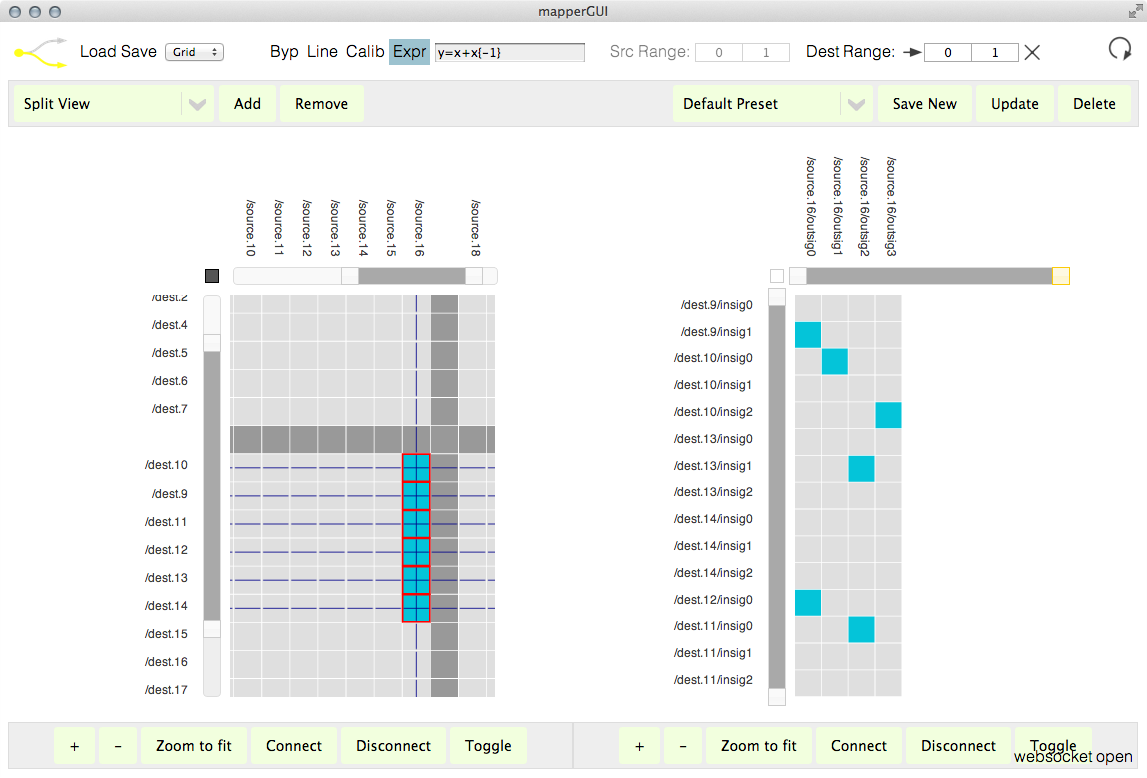
\includegraphics{figures/grid}}
\caption{The grid view}
\label{fig:grid}
\end{figure}

\begin{figure}[ht]
\centering
	\scalebox{0.4}{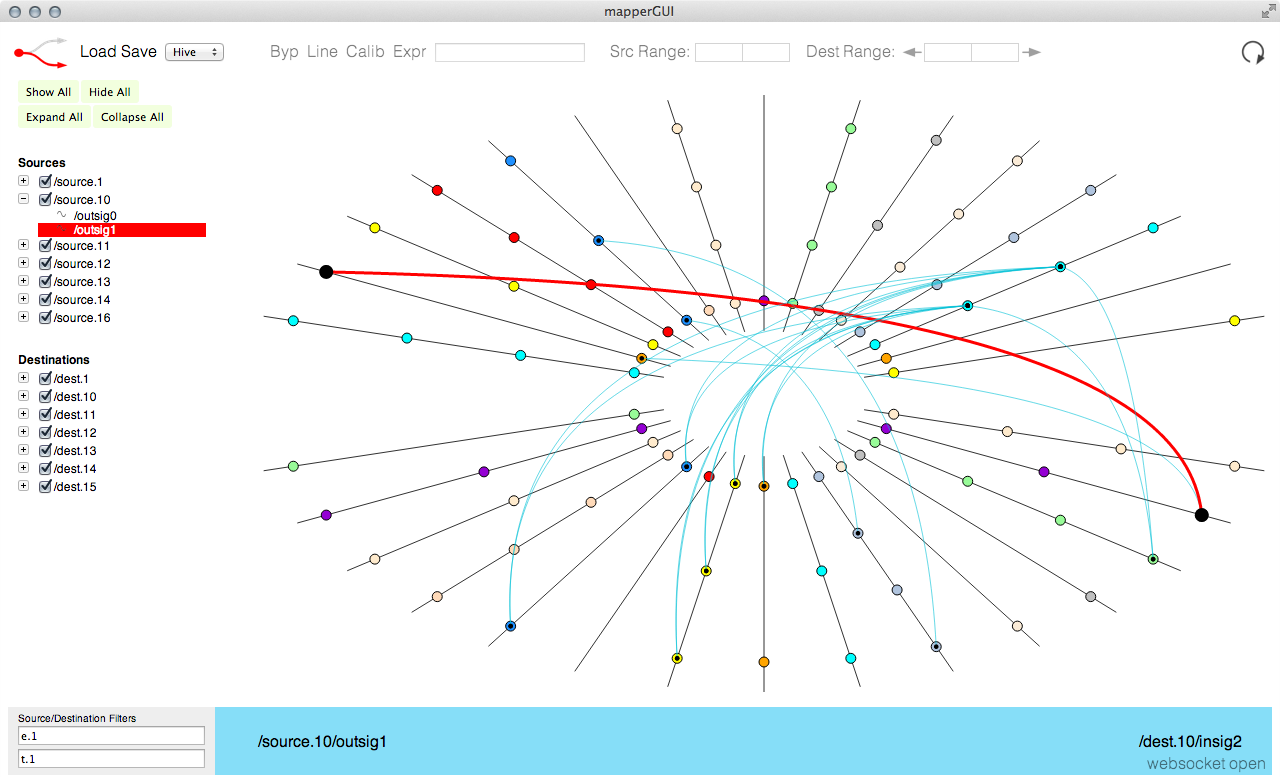
\includegraphics{figures/hive}}
\caption{The hive view}
\label{fig:hive}
\end{figure}

	
\section{User Centric Design}
	use cases

\section{Robustness and Responsiveness}
	speed tests

\section{Creation of a Standalone}